% Abdelwadoud Mabrouk
\documentclass[
  11pt,
  a4paper,
  oneside,
  headings=normal,
  parskip=half,
  DIV=12
]{scrreprt}

\usepackage[T1]{fontenc}
\usepackage[utf8]{inputenc}
\usepackage[ngerman]{babel}
\usepackage{csquotes}
\usepackage{lmodern}
\usepackage{microtype}
\usepackage{geometry}
\usepackage{setspace}
\usepackage{xcolor}
\usepackage{graphicx}
\usepackage{float}
\usepackage{booktabs}
\usepackage{tabularx}
\usepackage{array}
\usepackage{enumitem}
\usepackage{hyperref}
\usepackage{xurl}
\usepackage{scrlayer-scrpage}
\usepackage[backend=biber,style=numeric]{biblatex}

\addbibresource{literatur.bib}

\geometry{left=3cm,right=2.5cm,top=2.7cm,bottom=2.7cm}
\onehalfspacing

\hypersetup{
  colorlinks=true,
  linkcolor=blue!60!black,
  citecolor=blue!60!black,
  urlcolor=blue!60!black,
  pdftitle={Microservice-Architektur eines Möbel-Online-Shops},
  pdfauthor={Abdelwadoud Mabrouk, Mohammed Amine Grioui}
}

\pagestyle{scrheadings}
\clearpairofpagestyles
\ihead{Möbel-Online-Shop -- Abschlussbericht}
\ohead{\headmark}
\cfoot{\pagemark}

\newcommand{\projektname}{Microservice-orientierter Möbel-Online-Shop}
\newcommand{\modulname}{Vertiefung Software Engineering}
\newcommand{\hochschule}{Fachhochschule Südwestfalen}
\newcommand{\dozent}{Prof. Dr.-Ing. Doga Arinir}
\newcommand{\semester}{Sommersemester 2026}
\newcommand{\autoreneins}{Abdelwadoud Mabrouk}
\newcommand{\autorenzwei}{Mohammed Amine Grioui}
\newcommand{\frontendname}{WohnWerk}

\begin{document}

\hypersetup{pageanchor=false}
\begin{titlepage}
  \centering
  {\Large \hochschule \par}
  \vspace{0.7cm}
  {\large Fachbereich Informatik und Naturwissenschaften \par}
  \vspace{1.7cm}

  {\LARGE \textbf{Abschlussbericht} \par}
  \vspace{0.5cm}
  {\Large im Modul \modulname \par}
  \vspace{1.4cm}

  {\huge \textbf{Microservice-Architektur} \par}
  \vspace{0.2cm}
  {\huge \textbf{eines Möbel-Online-Shops} \par}
  \vspace{1.4cm}

  \renewcommand{\arraystretch}{1.25}
  \begin{tabular}{>{\bfseries}ll}
    Projekt: & \projektname \\
    Modul: & \modulname \\
    Dozent: & \dozent \\
    Semester: & \semester \\
    Autoren: & \autoreneins, \autorenzwei \\
    Abgabedatum: & 6. September 2026
  \end{tabular}

  \vfill
  \IfFileExists{../images/logo_Hochschule.png}
    {
\includegraphics[width=0.22\textwidth]{../images/logo_Hochschule.png}}{}
\end{titlepage}

\hypersetup{pageanchor=true}
\pagenumbering{Roman}
\tableofcontents
\clearpage
\pagenumbering{arabic}

\chapter*{Kurzfassung}
\addcontentsline{toc}{chapter}{Kurzfassung}

Gegenstand dieser Arbeit ist die Konzeption und Implementierung einer verteilten E-Commerce-Plattform für den Möbelhandel. Die Systemarchitektur basiert auf dem Paradigma der Microservices im Kontext des Domain-Driven Designs (DDD), wobei jeder Dienst die vollständige Datenhoheit über seine Domäne behält.

Zur Kopplung der Dienste wird ein hybrider Kommunikationsansatz gewählt: Synchrone REST-Schnittstellen kommen dort zum Einsatz, wo unmittelbare Rückmeldungen erforderlich sind, während eine ereignisgesteuerte Architektur (EDA) auf Basis von Apache Kafka die asynchrone Benachrichtigung und die Orchestrierung verteilter Transaktionen via Saga-Pattern übernimmt. Das Frontend wurde als Single-Page-Application mit Angular realisiert.

Neben der technischen Umsetzung der Kernprozesse – von der Bestandsreservierung über die Zahlungsabwicklung bis hin zur Rechnungsgenerierung – liegt der Schwerpunkt auf der Resilienz des Gesamtsystems. Dies umfasst Mechanismen zur Vermeidung von Doppelverarbeitungen (Idempotenz), eine nachvollziehbare Audit-Timeline für Bestellzustände sowie ein definiertes Ausfall- und Kompensationsmanagement. Die Bereitstellung der Gesamtanwendung erfolgt containerisiert mittels Docker Compose.

\chapter{Problemstellung}

Aus Sicht des Endanwenders stellt ein Bestellvorgang in einem E-Commerce-System eine lineare und unkomplizierte Transaktion dar. Hinter der Benutzeroberfläche verbirgt sich jedoch ein komplexes Zusammenspiel mehrerer spezialisierter Teilsysteme. Der Gesamtprozess beschränkt sich nicht auf die Erfassung des Kaufwunsches, sondern umfasst die synchrone Prüfung und Reservierung von Warenbeständen, die Interaktion mit externen Zahlungsanbietern, die Erstellung steuerrelevanter Rechnungsdokumente sowie die Logistikabwicklung.

Die zentrale Herausforderung verteilter Architekturen (Microservices) liegt in der Erhaltung der zeitlichen und fachlichen Datenkonsistenz. Da Netzwerkverbindungen unzuverlässig sind und einzelne Dienste temporär ausfallen können, dürfen Teilausfälle nicht zu inkonsistenten Zuständen führen (beispielsweise einer erfolgten Bezahlung ohne entsprechende Bestandsreservierung).

Aus dieser Problemstellung ergeben sich folgende Kernanforderungen an das Gesamtsystem:
\begin{itemize}
    \item \textbf{Verteilte Transaktionssicherheit:} Sicherstellung, dass der Bestellprozess entweder vollständig erfolgreich durchläuft oder im Fehlerfall kontrolliert mittels Kompensationsmaßnahmen (Saga-Pattern) zurückgerollt wird.
    \item \textbf{Resilienz und Entkopplung:} Ausfälle einzelner Teilsysteme dürfen den gesamten Checkout-Prozess nicht blockieren oder Datenkorruption verursachen.
    \item \textbf{Idempotenz:} Schutz vor Mehrfachausführungen kritischer Operationen (wie doppelten Abbuchungen) bei Netzwerkwiederholungen (Retries).
\end{itemize}

\section{Bestellprozess}

Der Bestellprozess erfordert eine sequenzielle Orchestrierung der beteiligten Domänendienste: Nach der Absendung der Bestellung durch den Kunden prüft und reserviert der Warenwirtschaftsdienst (\textit{Warehouse}) den Bestand. Erst nach erfolgreicher Reservierung verarbeitet der Abrechnungsdienst (\textit{Billing}) die Zahlung, woraufhin der Lagerbestand endgültig abgebucht und die Rechnung (\textit{Invoice}) generiert wird. Jeder Prozessschritt dient als strikte Voraussetzung für den nachfolgenden.

Im Fehlerfall greifen definierte Kompensationsmechanismen: Bei unzureichendem Bestand wird der Zahlungsvorgang gar nicht erst initiiert. Schlägt die Bezahlung fehl, wird die Bestandsreservierung automatisch wieder freigegeben. Ein Fehlschlagen der Rechnungsstellung hingegen löst eine kontrollierte Wiederholung (\textit{Retry}) aus, ohne die vorausgegangene Transaktion abzubrechen.


\section{Architekturtreiber und Domänentrennung}

Die Kerndomänen – \textbf{Bestellabwicklung, Lagerhaltung, Zahlungsabwicklung, Rechnungsstellung und Auditierung} – unterliegen unterschiedlichen fachlichen Änderungszyklen und Skalierungsanforderungen. Eine monolithische Architektur mit gemeinsamer Datenhaltung würde zu einer starken Kopplung führen. Gemäß dem Domain-Driven Design (DDD) wurden daher klare Domänengrenzen (\textit{Bounded Contexts}) mit eigener Datenhoheit definiert.

Diese Verteilung erfordert die Lösung klassischer Herausforderungen verteilter Systeme:
\begin{itemize}
    \item \textbf{Hybride Kommunikation:} Die Wahl zwischen synchronen Anfragen (REST) für direkte Ausführungsentscheidungen und asynchroner Event-Übertragung (Kafka) für entkoppelte Benachrichtigungen.
    \item \textbf{Zustands-Entkopplung und Idempotency:} Die sichere Handhabung von Netzwerk-Wiederholungen und redundanten Event-Eingängen.
    \item \textbf{Nachvollziehbarkeit:} Die lückenlose Rückverfolgbarkeit des Systemzustands über Service-Grenzen hinweg bei Fehlern.
\end{itemize}

\section{Zielsetzung und Abgrenzung}

Ziel dieser Arbeit ist die Entwicklung einer resilienten, verteilten E-Commerce-Architektur mit transparenten Domänengrenzen, deterministischem Fehlerhandling sowie automatisiert reproduzierbaren Tests. Das Gesamtsystem soll als lokal lauffähiger Stack mittels Docker Compose orchestriert werden.

Als Abgrenzung im Rahmen dieses Hochschulprojekts gilt: Der produktive Einsatz von externen Identity Providern (IAM), hochverfügbaren Cluster-Infrastrukturen (HA), professionellem Secret-Management sowie die Zertifizierung echter Zahlungsanbieter (z.\,B. PCI-DSS) sind nicht Gegenstand dieser Implementierung und markieren den Ausblick für ein Production-Engineering.


\chapter{Lösungskonzept und Systemarchitektur}

Ausgehend von den definierten Anforderungen und Problemstellungen beschreibt dieses Kapitel die Architektur der entwickelten Gesamtlösung. Der Fokus liegt zunächst auf der Strukturierung der einzelnen Microservices und ihrer hybriden Kommunikationsinfrastruktur. Anschließend werden sowohl der reguläre Transaktionsablauf im Erfolgsfall als auch die verankerten Fehlertoleranz- und Kompensationsmechanismen detailliert evaluiert.

\section{Services und Gesamtarchitektur}

Die Anwendung ist in fünf fachlich getrennte Microservices aufgeteilt:

\begin{itemize}[leftmargin=1.2cm]
  \item Der Shop-Service verwaltet Bestellungen sowie Produkte und orchestriert den Bestellprozess. Obwohl der Produkt-Katalog nach Domain-Driven Design (DDD) einen eigenen Bounded Context bildet, wird er vorerst als isoliertes Modul im Shop-Service betrieben (com.vseonlineshop.shopservice.product). Dies spart Infrastrukturkosten, Netzwerk-Latenzen und Pipeline-Komplexität. Dank strikter Trennung auf Code-Ebene bleibt die Auslagerung in einen eigenständigen Microservice im Sinne einer Evolutionary Architecture jederzeit möglich.
  \item Der Warehouse-Service verwaltet Lagerbestand und Reservierungen.
  \item Der Billing-Service verarbeitet Zahlungen über externe Zahlungsanbieter.
  \item Der Invoice-Service erstellt Rechnungen.
  \item Der Audit-Service speichert die fachliche Historie aller relevanten Ereignisse.
\end{itemize}

Die Aufteilung in fachlich getrennte Microservices verfolgt das Ziel, Verantwortlichkeiten klar voneinander zu trennen. Shop-, Billing-, Warehouse- und Audit-Service besitzen jeweils eine eigene PostgreSQL-Datenbank. Der Invoice-Service verwaltet seine Rechnungsdaten und PDF-Dokumente dateibasiert in einem eigenen Docker-Volume. Dadurch entstehen eine geringe Kopplung zwischen den Komponenten sowie die Möglichkeit, einzelne Services unabhängig weiterzuentwickeln, zu testen und bereitzustellen. Dieses Database-per-Service-Prinzip folgt der fachlichen Trennung von Microservices \cite{fowlerMicroservices}.

Die folgende Abbildung zeigt die Gesamtarchitektur des Systems. Sie verdeutlicht die Verantwortlichkeiten der einzelnen Services, die Kommunikation über REST und Kafka sowie das Database-per-Service-Prinzip.

\begin{figure}[H]
  \centering
  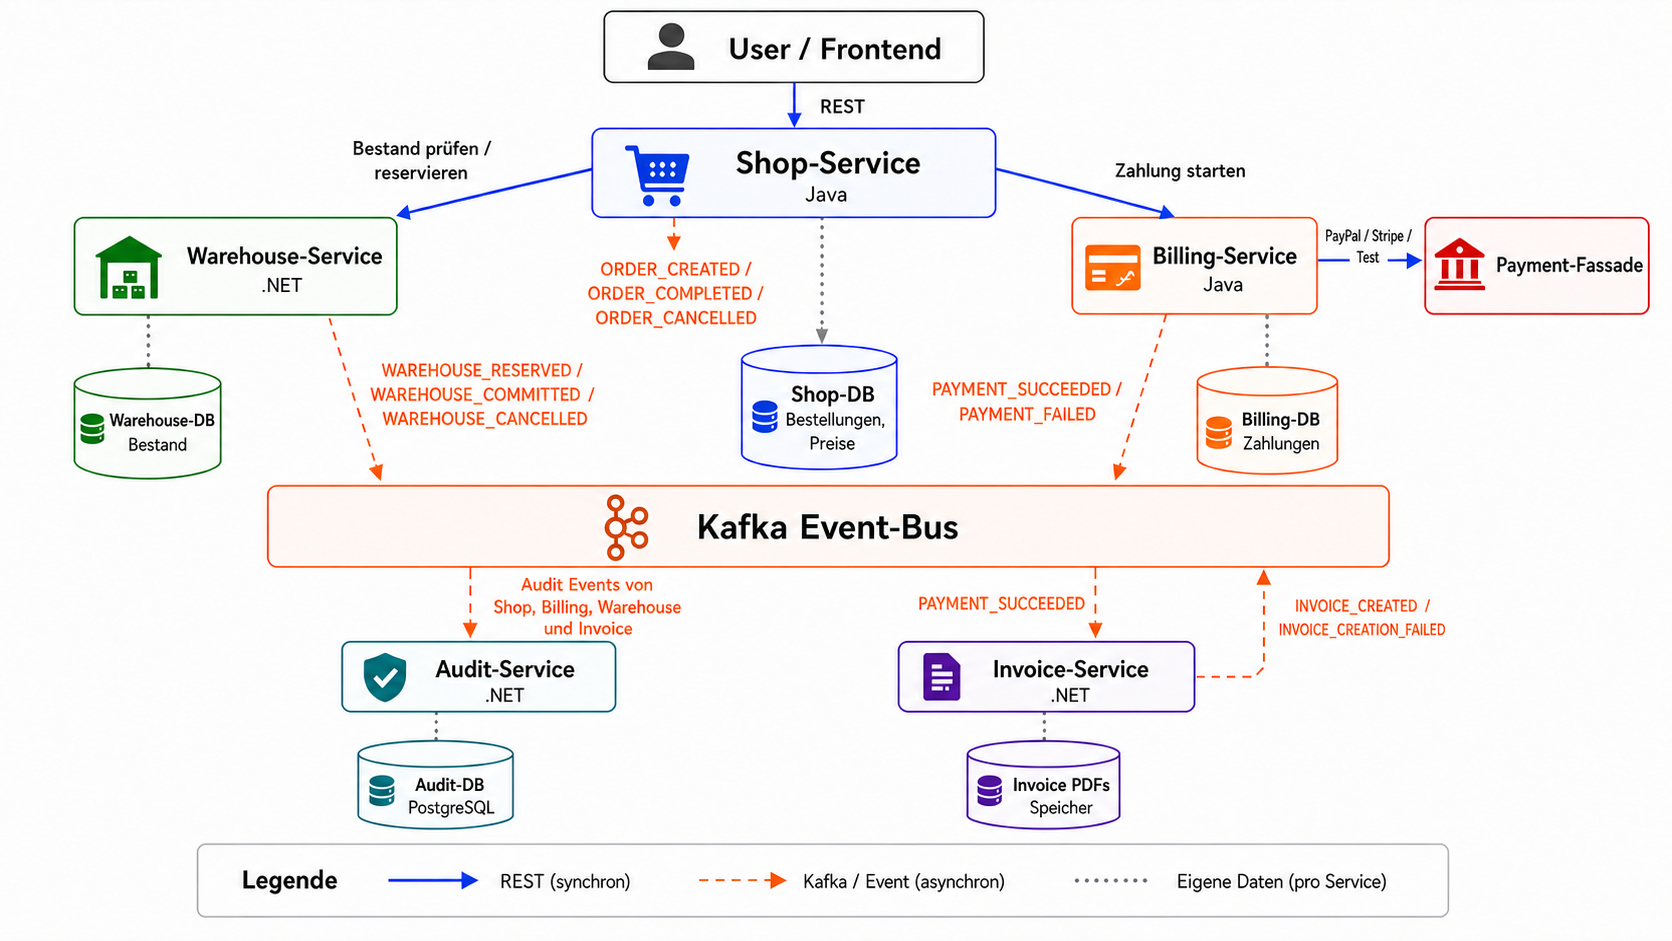
\includegraphics[width=0.94\textwidth]{../images/system-architecture-overview.png}
  \caption{Gesamtarchitektur des Möbel-Online-Shops mit REST-Kommunikation, Kafka-Ereignissen und Database-per-Service-Prinzip}
  \label{fig:gesamtarchitektur}
\end{figure}

Abbildung~\ref{fig:gesamtarchitektur} zeigt außerdem die Payment-Fassade. Weitere Architekturentscheidungen sowie ADRs befinden sich in der separaten Datei \emph{docs/architecture.md}. Dieser Bericht konzentriert sich auf die wesentlichen Konzepte sowie deren Umsetzung.


\section{Kommunikationsstrategie und Transaktionssteuerung}

Für die Interaktion zwischen den Microservices wird ein hybrider Ansatz aus synchroner REST-Kommunikation und asynchroner Ereignisverarbeitung mittels Apache Kafka eingesetzt.

Synchrone REST-Schnittstellen kommen dort zum Einsatz, wo der initiierende Service unmittelbar eine Ausführungsentscheidung benötigt. Dies betrifft insbesondere die Bestandsreservierung im Warenwirtschaftsdienst sowie die Auslösung von Zahlungstransaktionen. Durch das synchrone Antwortverhalten kann der aufrufende Dienst den Prozessfluss direkt fortsetzen oder bei Fehlern unmittelbar abbrechen.

Die Wahl einer synchronen REST-Schnittstelle für die Zahlungsinitialisierung erfolgt dabei bewusst: Nach der Vorbereitung der Transaktion liefert der Abrechnungsdienst (\textit{Billing-Service}) direkt die Checkout-URL des Zahlungsanbieters zurück. Diese wird umgehend an die Benutzeroberfläche weitergeleitet, um dem Endanwender eine unterbrechungsfreie Interaktion zu ermöglichen. Eine asynchrone Ereignisverarbeitung an dieser Stelle würde komplexe Polling-Mechanismen im Client erfordern und die Latenz unnötig erhöhen.

Apache Kafka wird demgegenüber für domänenspezifische Ereignisse (\textit{Domain Events}) genutzt, deren Verarbeitung entkoppelt und ohne Blockierung des Hauptprozesses erfolgen kann \cite{apacheKafka}. Nachgelagerte Dienste wie der Rechnungsdienst (\textit{Invoice-Service}) oder das Audit-System konsumieren diese Ereignisse autonom, ohne dass der Sender auf eine Bestätigung warten muss.

Da in dieser verteilten Architektur keine datenbankübergreifenden ACID-Transaktionen existieren, wird der Gesamtablauf nach dem \textit{Saga-Pattern} (Orchestration) gesteuert. Jeder beteiligte Dienst führt Operationen ausschließlich lokal auf seiner eigenen Datenbasis aus.

Beim Auftreten von Fehlern während des Checkouts greift eine kaskadierende Kompensationslogik: Über dedizierte Kafka-Ereignisse (beispielsweise \texttt{OrderCancelled}) werden bereits erfolgreich durchlaufene Teilschritte in umgekehrter Reihenfolge fachlich zurückgerollt. Schlägt etwa die Bezahlung fehl, veranlasst das emittierte Event den Warenwirtschaftsdienst zur expliziten Freigabe der zuvor reservierten Lagerbestände.

\section{Payment-Fassade und asynchrone Webhook-Verarbeitung}

\subsection{Payment-Fassade}

Der Billing-Service kapselt externe Zahlungsanbieter hinter einer gemeinsamen Schnittstelle (Payment-Fassade). Der Shop-Service kennt die konkrete Implementierung des jeweiligen Anbieters nicht und kommuniziert ausschließlich mit dem Billing-Service. Die Anbindung erfolgt über ein gemeinsames Interface, das grundlegende fachliche Operationen (wie die Initialisierung oder den Abschluss einer Zahlung) definiert. Die konkrete Implementierung wird zur Laufzeit anhand des ausgewählten Anbieters bestimmt. Dieses Vorgehen entspricht dem Strategy Pattern und ermöglicht es, das System um weitere Provider zu ergänzen, ohne bestehende Komponenten ändern zu müssen.

\subsection{Auswahl der Zahlungsanbieter}

Zur Validierung der Architektur wurden mit PayPal und Stripe die zwei weltweit führenden Zahlungsdienstleister gewählt. Im Vergleich zu Alternativen wie Klarna, das primär auf Buy-Now-Pay-Later (Kauf auf Rechnung bzw. Ratenkauf) spezialisiert ist und dadurch verzögerte Bonitätsprüfungen sowie komplexe, mehrtägige Zustandsautomaten erzwingt, decken Stripe und PayPal neben einer globalen Marktabdeckung die beiden wichtigsten synchronen bis leicht-asynchronen Integrationsmuster des E-Commerce ab.

\begin{itemize}
    \item \textbf{Stripe} repräsentiert den Industriestandard für direkte Kreditkarten- und Wallet-Zahlungen mit einem stark Webhook-getriebenen Ereignismodell.

    \item \textbf{PayPal} kombiniert das Wallet-Prinzip mit einem zweistufigen Integrationsmodell aus Autorisierung (\textit{Intent}) und explizitem Bestätigungsschritt (\textit{Capture}).
\end{itemize}

\subsection{Webhook-Verarbeitungsprozess}

Da die Zahlungsabwicklung auf den externen Systemen der Zahlungsanbieter (z.\,B. PayPal) erfolgt, dient der \textit{Billing-Service} als zentrales Inbound-Gateway für eingehende Statusbenachrichtigungen (Webhooks). Sobald eine Transaktion durch den Endanwender freigegeben wurde, benachrichtigt der jeweilige Provider den \textit{Billing-Service} über einen definierten HTTP-POST-Endpunkt.

Der Prozess übersetzt die externe Benachrichtigung in die interne Event-Driven Architecture:

\begin{itemize}
    \item \textbf{Statusaktualisierung \& Event-Übersetzung:} Der \textit{Billing-Service} verarbeitet die eingehende Benachrichtigung, aktualisiert den lokalen Zahlungsstatus und transformiert die Nachricht in ein internes Domänen-Ereignis (\texttt{PaymentSucceeded} bzw. \texttt{PaymentFailed}).
    \item \textbf{Asynchrone Event-Distribution:} Das Domänen-Ereignis wird auf das Kafka-Topic \texttt{billing} publiziert. Dadurch werden nachgelagerte Dienste (Shop-Service für den Order-Abschluss, Audit-Service zur Protokollierung und Invoice-Service zur Rechnungsgenerierung) vollständig entkoppelt informiert.
    \item \textbf{Lokale Webhook-Entwicklung (PayPal vs. Stripe):} Für das Testen der Webhooks in der lokalen Entwicklungs- und Docker-Umgebung kommen provider-spezifische Ansätze zum Einsatz:
    \begin{itemize}
        \item \textit{PayPal:} Für externe Sandbox-Webhooks kann optional ein ngrok-Tunnel über das Docker-Compose-Profil external-webhooks gestartet werden. Der lokale Standard-Stack funktioniert ohne diesen Tunnel.
        \item \textit{Stripe:} Hier wird die herstellereigene Entwickler-CLI (\textit{Stripe CLI}) verwendet, die Ereignisse direkt lokal abfängt und ohne externen Tunnel an den Service weiterleitet.
    \end{itemize}
\end{itemize}



\section{Erfolgreicher Bestellprozess}

Ein Kunde startet den Checkout. Der Shop-Service erstellt zunächst die Bestellung und veröffentlicht das Ereignis \texttt{ORDER\_CREATED}. Anschließend reserviert der Warehouse-Service die angeforderten Artikel und veröffentlicht \texttt{WAREHOUSE\_RESERVED}. Erst danach wird die Zahlung über den Billing-Service gestartet.

Nach erfolgreichem Abschluss der Zahlung veröffentlicht der Billing-Service das Ereignis \texttt{PAYMENT\_SUCCEEDED}. Parallel führt der Shop-Service den Warehouse-Commit durch. Erst nachdem der Warehouse-Service den erfolgreichen Commit mit \texttt{WAREHOUSE\_COMMITTED} bestätigt hat, schließt der Shop-Service die Bestellung mit \texttt{ORDER\_COMPLETED} ab.

Der Happy Path besteht somit aus der folgenden Ereignisreihenfolge:

\begin{enumerate}
  \item \texttt{ORDER\_CREATED}
  \item \texttt{WAREHOUSE\_RESERVED}
  \item \texttt{PAYMENT\_INITIALIZED}
  \item \texttt{PAYMENT\_SUCCEEDED}
  \item \texttt{INVOICE\_CREATION\_STARTED}
  \item \texttt{INVOICE\_CREATED}
  \item \texttt{WAREHOUSE\_COMMITTED}
  \item \texttt{ORDER\_COMPLETED}
\end{enumerate}

Die folgende Abbildung zeigt den vollständigen Ablauf vom Checkout bis zum erfolgreichen Abschluss der Bestellung.

\begin{figure}[H]
  \centering
  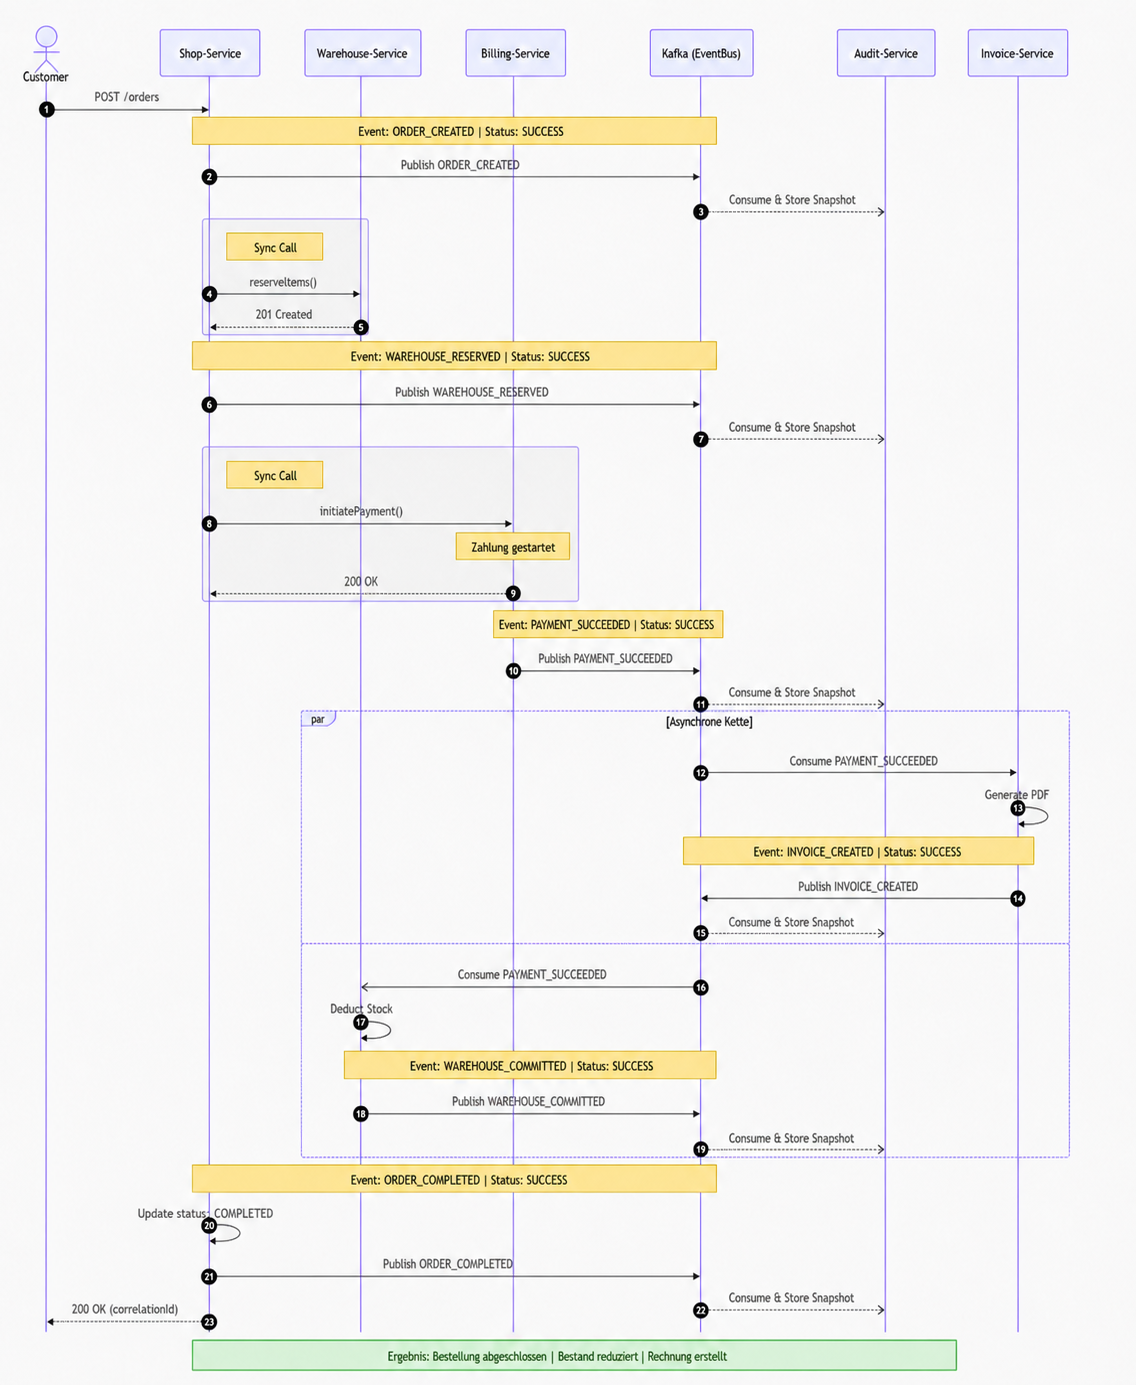
\includegraphics[width=0.90\textwidth,height=0.66\textheight,keepaspectratio]
    {../images/happy-path.png}
  \caption{Erfolgreicher Bestellprozess vom Checkout bis \texttt{ORDER\_COMPLETED}}
  \label{fig:happy-path}
\end{figure}

Abbildung~\ref{fig:happy-path} verdeutlicht außerdem, dass die Rechnungserstellung bewusst asynchron erfolgt. Nach der Veröffentlichung von \texttt{PAYMENT\_SUCCEEDED} kann der Invoice-Service unabhängig vom eigentlichen Checkout-Prozess arbeiten. Verzögerungen oder temporäre Fehler bei der Rechnungserstellung beeinflussen daher weder den erfolgreichen Zahlungsabschluss noch den Abschluss der Bestellung. Stattdessen werden Fehler über Retry-Mechanismen behandelt und zusätzlich durch den Audit-Service dokumentiert.

\textbf{Hinweis:} Das vollständige Sequenzdiagramm des Happy Paths befindet sich in der Datei \emph{docs/architecture.md} im Verzeichnis \texttt{docs}. Im Bericht wird aus Gründen der Lesbarkeit eine vereinfachte Darstellung verwendet.

\section{Fehlerfälle und Kompensation}

\subsection{Zahlung fehlgeschlagen}

Hat der \textit{Warehouse-Service} den Bestand bereits reserviert, meldet der \textit{Billing-Service} jedoch ein \texttt{PAYMENT\_FAILED}, veranlasst der \textit{Shop-Service} die Kompensation. Er emittiert das Ereignis \texttt{RESERVATION\_ROLLBACK\_REQUESTED} auf das Kafka-Topic. Daraufhin gibt der \textit{Warehouse-Service} die reservierten Artikel frei und bestätigt das erfolgreiche Rollback mit dem Event \texttt{WAREHOUSE\_RESERVATION\_CANCELLED}. Abschließend setzt der \textit{Shop-Service} den Bestellstatus auf \texttt{ORDER\_PAYMENT\_FAILED}. Mangels eines \texttt{PAYMENT\_SUCCEEDED}-Events wird durch den \textit{Invoice-Service} keine Rechnung generiert.

\begin{figure}[H]
  \centering
  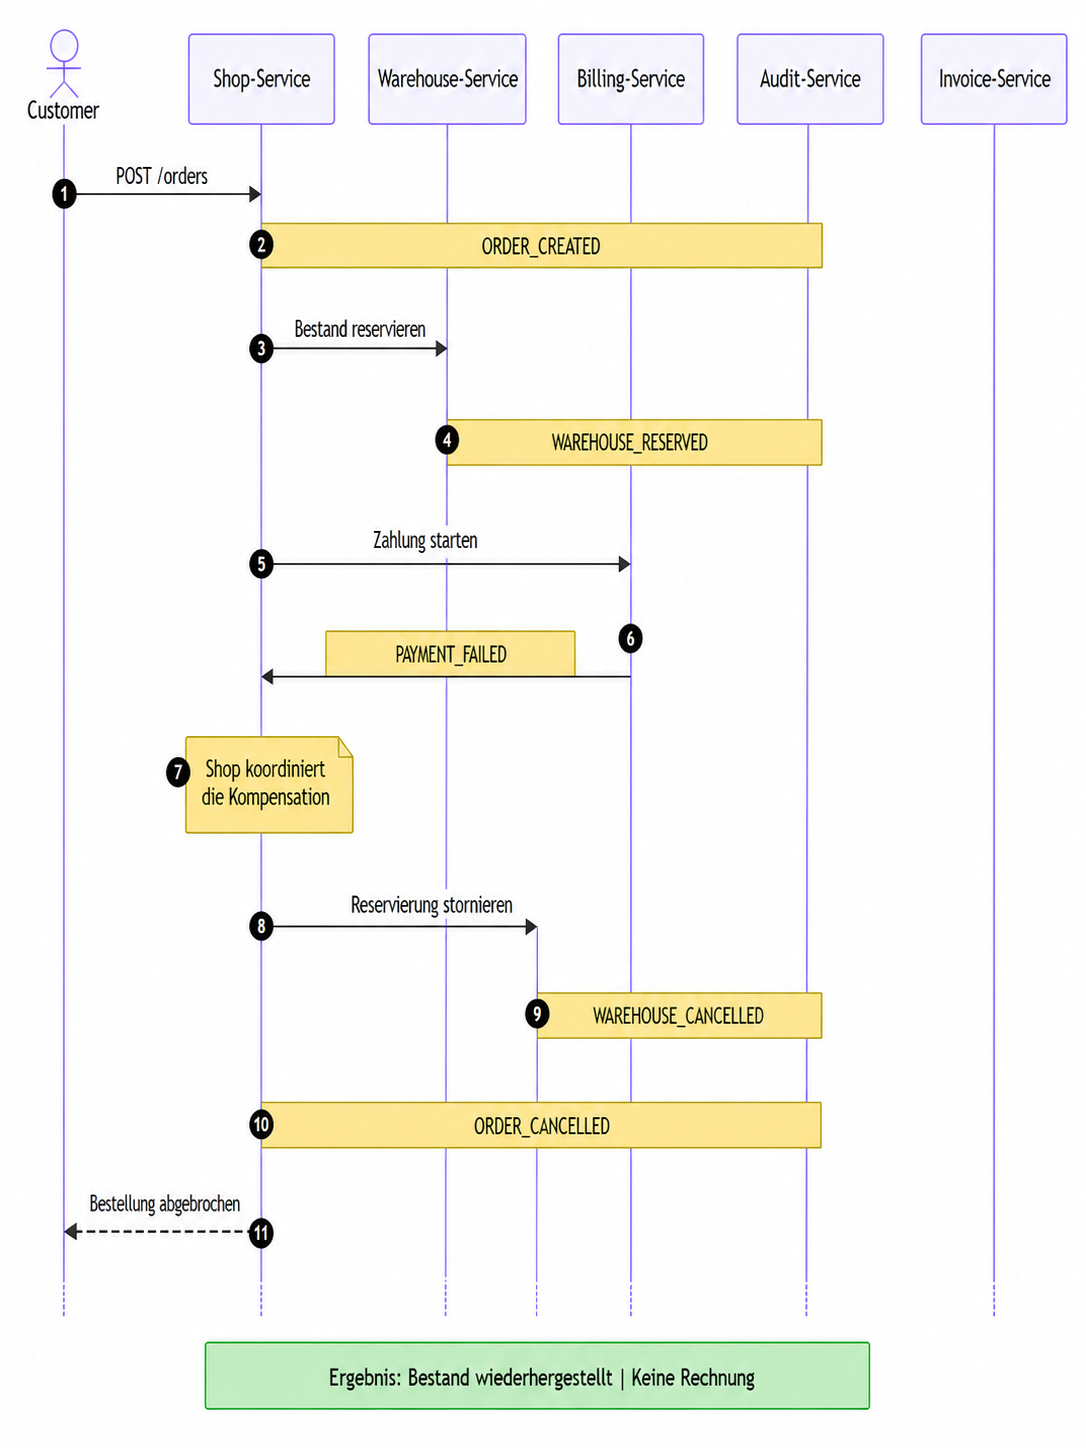
\includegraphics[width=0.78\textwidth,height=0.68\textheight,keepaspectratio]
    {../images/payment-failed-compensation.png}
  \caption{Kompensation einer Reservierung nach
  \texttt{PAYMENT\_FAILED}
  \label{fig:payment-failed}}
\end{figure}

\textbf{Hinweis:} Das vollständige Sequenzdiagramm zur fehlgeschlagenen Zahlung ist in \texttt{docs/architecture.md} dokumentiert. Im Bericht wird aus Gründen der Lesbarkeit eine vereinfachte Darstellung verwendet.

\subsection{Bestand nicht verfügbar}

Reicht der Bestand nicht aus, antwortet Warehouse mit
\texttt{409 Conflict} und dokumentiert
\texttt{WAREHOUSE\_OUT\_OF\_STOCK}. Der Shop bricht die Bestellung
kontrolliert mit \texttt{ORDER\_OUT\_OF\_STOCK} ab. Weil keine Reservierung
entsteht, folgen weder Zahlung noch Commit oder Rechnung. Der Bestand bleibt
unverändert. Dieser Ablauf ist ein kontrollierter Abbruch und keine
Kompensation.

\begin{figure}[H]
  \centering
  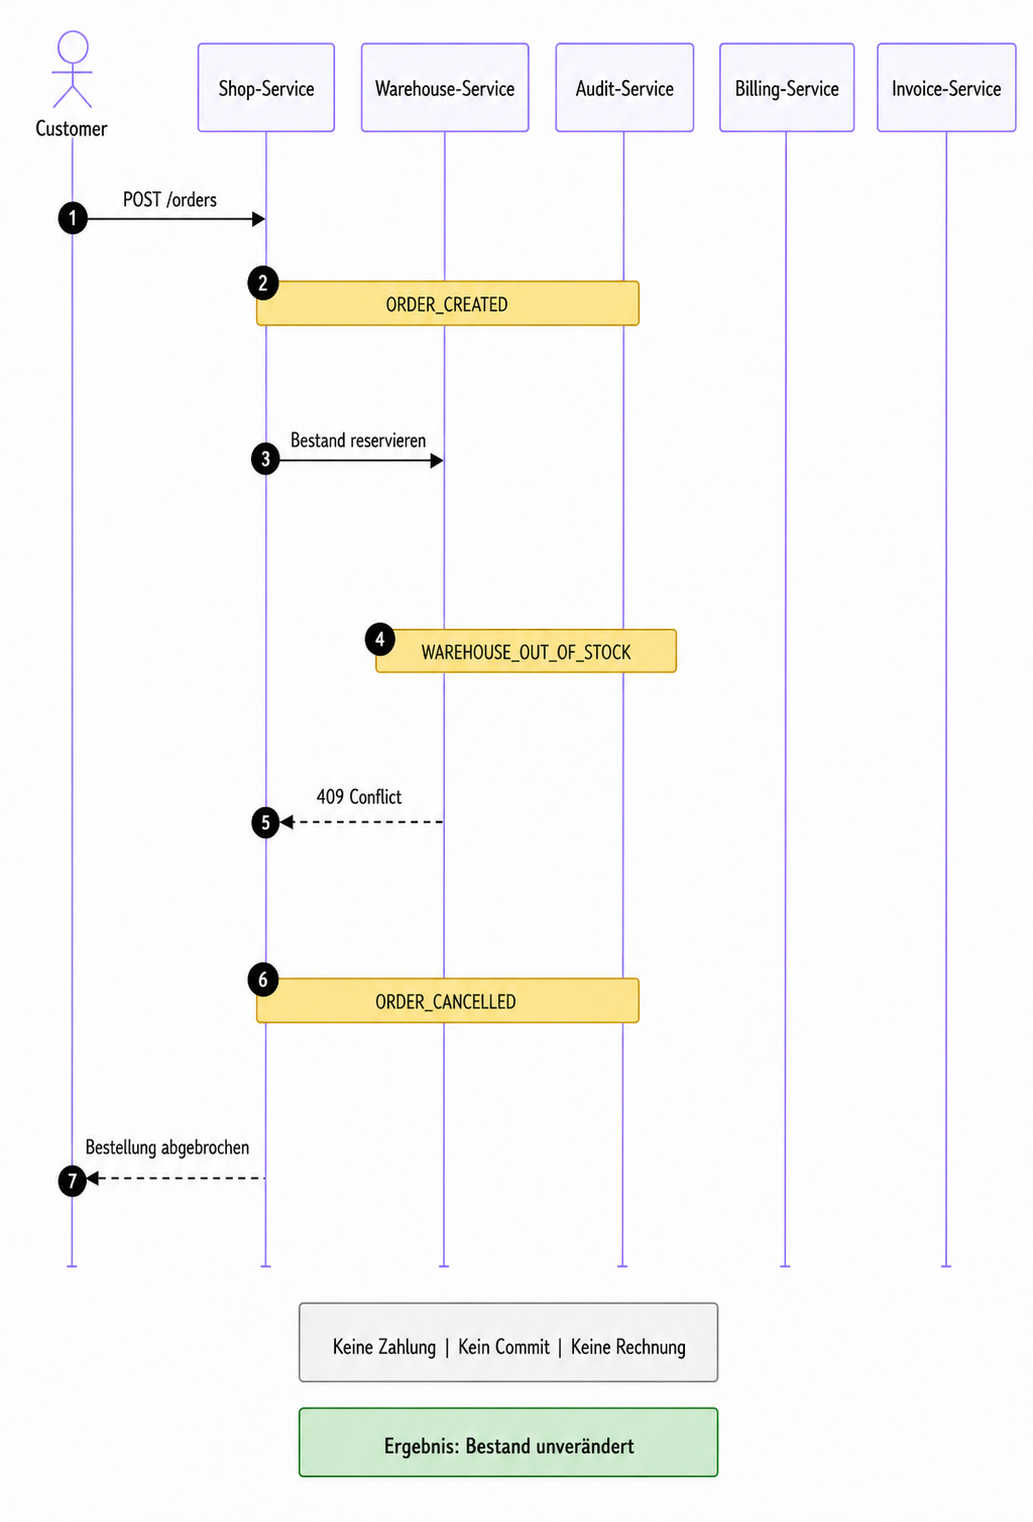
\includegraphics[width=0.74\textwidth,height=0.66\textheight,keepaspectratio]
    {../images/warehouse-out-of-stock.png}
  \caption{Kontrollierter Bestellabbruch bei nicht verfügbarem Bestand
  \label{fig:out-of-stock}}
\end{figure}

\subsection{Kompensationsszenario: Ausfall des Warehouse-Services beim Commit}

Das Szenario illustriert das Zusammenspiel aus Resilience4j-Retry, synchroner Kompensation und asynchroner Eventual Consistency bei einem Ausfall des Warehouse-Services während des Commit-Schritts.

\begin{enumerate}
    \item \textbf{Ausgangslage \& Retry-Logik:}
    Nach erfolgreicher Zahlung (\texttt{PaymentSucceeded}) erzeugt der \textit{Invoice-Service} die Rechnung. Der \textit{Shop-Service} versucht anschließend, den reservierten Bestand synchron über den REST-Endpunkt \texttt{/commit} abzubuchen. Bei Ausfällen (\texttt{ResourceAccessException}, \texttt{HttpServerErrorException}) greift eine \textit{Resilience4j}-Retry-Logik (\texttt{max-attempts=3}, Initialverzögerung: $1\,\mathrm{s}$, Multiplikator: $2$).

 \item \textbf{Saga-Kompensation \& Rollback:}
Bleiben alle Wiederholungsversuche erfolglos, leitet der \textit{Shop-Service} die Kompensations-Saga ein:
\begin{itemize}
    \item \textbf{Fehlersignalisierung:} Das System signalisiert den fehlgeschlagenen Warenausgang asynchron an die beteiligten Komponenten.
    \item \textbf{Synchroner Payment-Refund:} Der \textit{Shop-Service} stößt direkt eine synchrone Rückerstattung beim \textit{Billing-Service} an.
    \item \textbf{Saga-Abschluss:} Nach erfolgreicher Bestätigung der Rückabwicklung wird der lokale Transaktionszustand finalisiert und das finale Kompensations-Event publiziert.
\end{itemize}
\end{enumerate}


\textbf{Rechnungserstellung fehlgeschlagen.}

Erreicht \texttt{PAYMENT\_SUCCEEDED} den Invoice-Service, startet die
Rechnungserstellung asynchron. Schlägt das Schreiben der PDF-Datei fehl,
versucht der Service den Vorgang insgesamt dreimal. Die erfolgreiche Zahlung
und der Warehouse-Commit werden dabei nicht rückgängig gemacht. Bleiben alle
Versuche erfolglos, dokumentiert Invoice
\texttt{INVOICE\_CREATION\_FAILED} im Audit-Service. Eine doppelt zugestellte
Nachricht erzeugt wegen der \texttt{transactionId} keine zweite Rechnung.


\subsection{Auditierung und Idempotenz}

Die Correlation-ID verknüpft alle Teilschritte einer Bestellung serviceübergreifend zu einer chronologischen Timeline im Audit-Service. Eindeutige \texttt{eventId}s sowie die automatische Verkettung über \texttt{previousEventId} gewährleisten eine lückenlos nachvollziehbare Prozesskette.

Um Doppelverarbeitungen infolge von Netzwerkwiederholungen, Kafka-Re-Delivery oder mehrfach zugestellten Webhooks zu vermeiden, implementiert das System einen mehrstufigen Idempotenz-Schutz:

\begin{description}
    \item[Frontend (UI-Shielding):]
    Der Checkout-Button wird unmittelbar nach dem Klick deaktiviert, sodass Mehrfachanfragen durch den Benutzer verhindert werden.

    \item[Billing-Service:]
    Eingehende Webhooks (PayPal und Stripe) werden anhand der vom Zahlungsanbieter mitgelieferten Metadaten auf Duplikate geprüft. Bereits verarbeitete Webhooks werden verworfen.

    \item[Warehouse-Service:]
    Eine \texttt{orderId} erzeugt genau eine Lagerreservierung. Wiederholte Aufrufe der Endpunkte \texttt{/commit} oder \texttt{/cancel} führen zu keiner erneuten Änderung des Lagerbestands.

    \item[Invoice-Service:]
    Für jede \texttt{paymentId} wird genau eine PDF-Rechnung erzeugt.

    \item[Audit-Service:]
    Ereignisse mit einer bereits bekannten \texttt{eventId} werden ignoriert, wodurch eine doppelte Protokollierung ausgeschlossen wird.
\end{description}


\chapter{Umsetzung}

Nachdem die Architektur feststand, haben wir die Bausteine schrittweise
umgesetzt. Dieses Kapitel beschreibt nur die Teile, die für das Verständnis des
Systems wichtig sind. Weitere technische Details und ADRs stehen in
\emph{docs/architecture.md}.

\begin{table}[H]
  \centering
  \caption{Technologien des Projekts
  \label{tab:technologien}}
  \begin{tabularx}{0.88\textwidth}{>{\bfseries}p{3.2cm}X}
    \toprule
    Bereich & Technologie \\
    \midrule
    Frontend & Angular 22 \\
    Backend & Spring Boot und .NET 10 \\
    Messaging & Apache Kafka \\
    Datenbanken & PostgreSQL \\
    Container & Docker Compose \\
    Webserver & Nginx \\
    Observability & OpenTelemetry, Loki und Grafana \\
    \bottomrule
  \end{tabularx}
\end{table}

\section{Backend}

Die Backend-Architektur ist als polyglottes Microservice-System aufgebaut: Während der Shop-Service und der Billing-Service auf Java mit Spring Boot basieren, sind der Warehouse-Service, der Invoice-Service und der Audit-Service in .NET 10 implementiert. Protokolle und Standards wie REST, Apache Kafka und JSON gewährleisten die technologieunabhängige Entkopplung und Interoperabilität zwischen beiden Ökosystemen.

\section{Benutzeroberfläche und Rollenkonzept}

Das Frontend bildet als gemeinsame Oberfläche das zentrale Bindeglied zwischen den Endanwendern und der verteilten Systemarchitektur. Es visualisiert den Zustand der Microservices, während die gesamte fachliche Logik strikt in den nachgelagerten Backend-Diensten gekapselt bleibt.

Die Anwendung unterscheidet drei fachliche Verantwortungsbereiche:
\begin{itemize}
    \item \textbf{Kundenbereich:} Dient als primärer Einstiegspunkt für Stöber-, Bestell- und Bezahlvorgänge auf Basis des Produktkatalogs.
    \item \textbf{Lagerverwaltung (Warehouse):} Ermöglicht die Einsicht und Nachverfolgung von Bestandsreservierungen.
    \item \textbf{Administrations- und Auditbereich:} Bietet Einsicht in Rechnungsdokumente, protokollierte Systemereignisse sowie den übergreifenden Betriebsstatus der Services.
\end{itemize}

Angular Guards trennen die Demo-Rollen auf Ebene der Benutzeroberfläche. Der Audit-Adminbereich ist zusätzlich durch HTTP Basic Authentication geschützt; ein vollständiges serviceübergreifendes Berechtigungssystem ist jedoch nicht implementiert. Das agile Navigationskonzept unterstützt die Entkopplung der Domänen und macht den komplexen, verteilten Bestellablauf für die Nutzer transparent greifbar.

\begin{figure}[H]
  \centering
  
\includegraphics[width=0.94\textwidth,height=0.60\textheight,keepaspectratio]
    {../images/frontend-overview.png}
  \caption{Produktkatalog des Angular-22-Frontends \frontendname{} mit
  Navigation, Warenkorb, Kategorien und responsiver Produktübersicht
  \label{fig:frontend}}
\end{figure}
\section{Docker und Nginx}

Docker Compose startet Frontend, Services, Datenbanken, Kafka und Monitoring
reproduzierbar. Der gleiche Stack läuft dadurch auf verschiedenen
Entwicklungsrechnern mit derselben Konfiguration.

Nginx liefert den Angular-Produktionsbuild aus und leitet relative API-Pfade an
die zuständigen Services weiter. Das Frontend kennt keine internen
Container-Adressen.

\section{Technische Beobachtbarkeit und Monitoring}

Neben der fachlichen Nachvollziehbarkeit über das Audit-System erfordert die verteilte Architektur auch eine technische Beobachtbarkeit (\textit{Observability}). Um den Betriebsstatus aller Microservices zentral zu überwachen, wird eine Kombination aus Log-Aggregation und Telemetrie-Erfassung eingesetzt \cite{grafanaLoki}.

Aufgrund des polyglotten Technologiestacks und zur Optimierung des Implementierungsaufwands kommen zwei parallele Erfassungsstrategien zum Einsatz:

\begin{itemize}
    \item \textbf{.NET-Services:} Diese exportieren strukturierte Log- und Telemetriedaten nativ über den \textit{OpenTelemetry Collector}.
    \item \textbf{Spring-Boot-Services (\textit{Shop}, \textit{Billing}):} Um den Konfigurationsaufwand im zeitlich vorgegebenen Rahmen zu minimieren, werden deren JSON-Logs direkt über den \textit{Promtail}-Agenten aus den Docker-Containern ausgelesen und an Loki weitergeleitet.
\end{itemize}

Die gesammelten Logdaten werden im zentralen Log-Aggregationssystem \textit{Grafana Loki} konsolidiert und über \textit{Grafana}-Dashboards visualisiert. Durch die konsistente Mitführung einer eindeutigen \textit{Correlation-ID} über Service-Grenzen hinweg lassen sich fachliche Audit-Ereignisse nahtlos mit den technischen System-Logs korrelieren (siehe Abbildung~\ref{fig:monitoring}).

\begin{figure}[H]
  \centering
  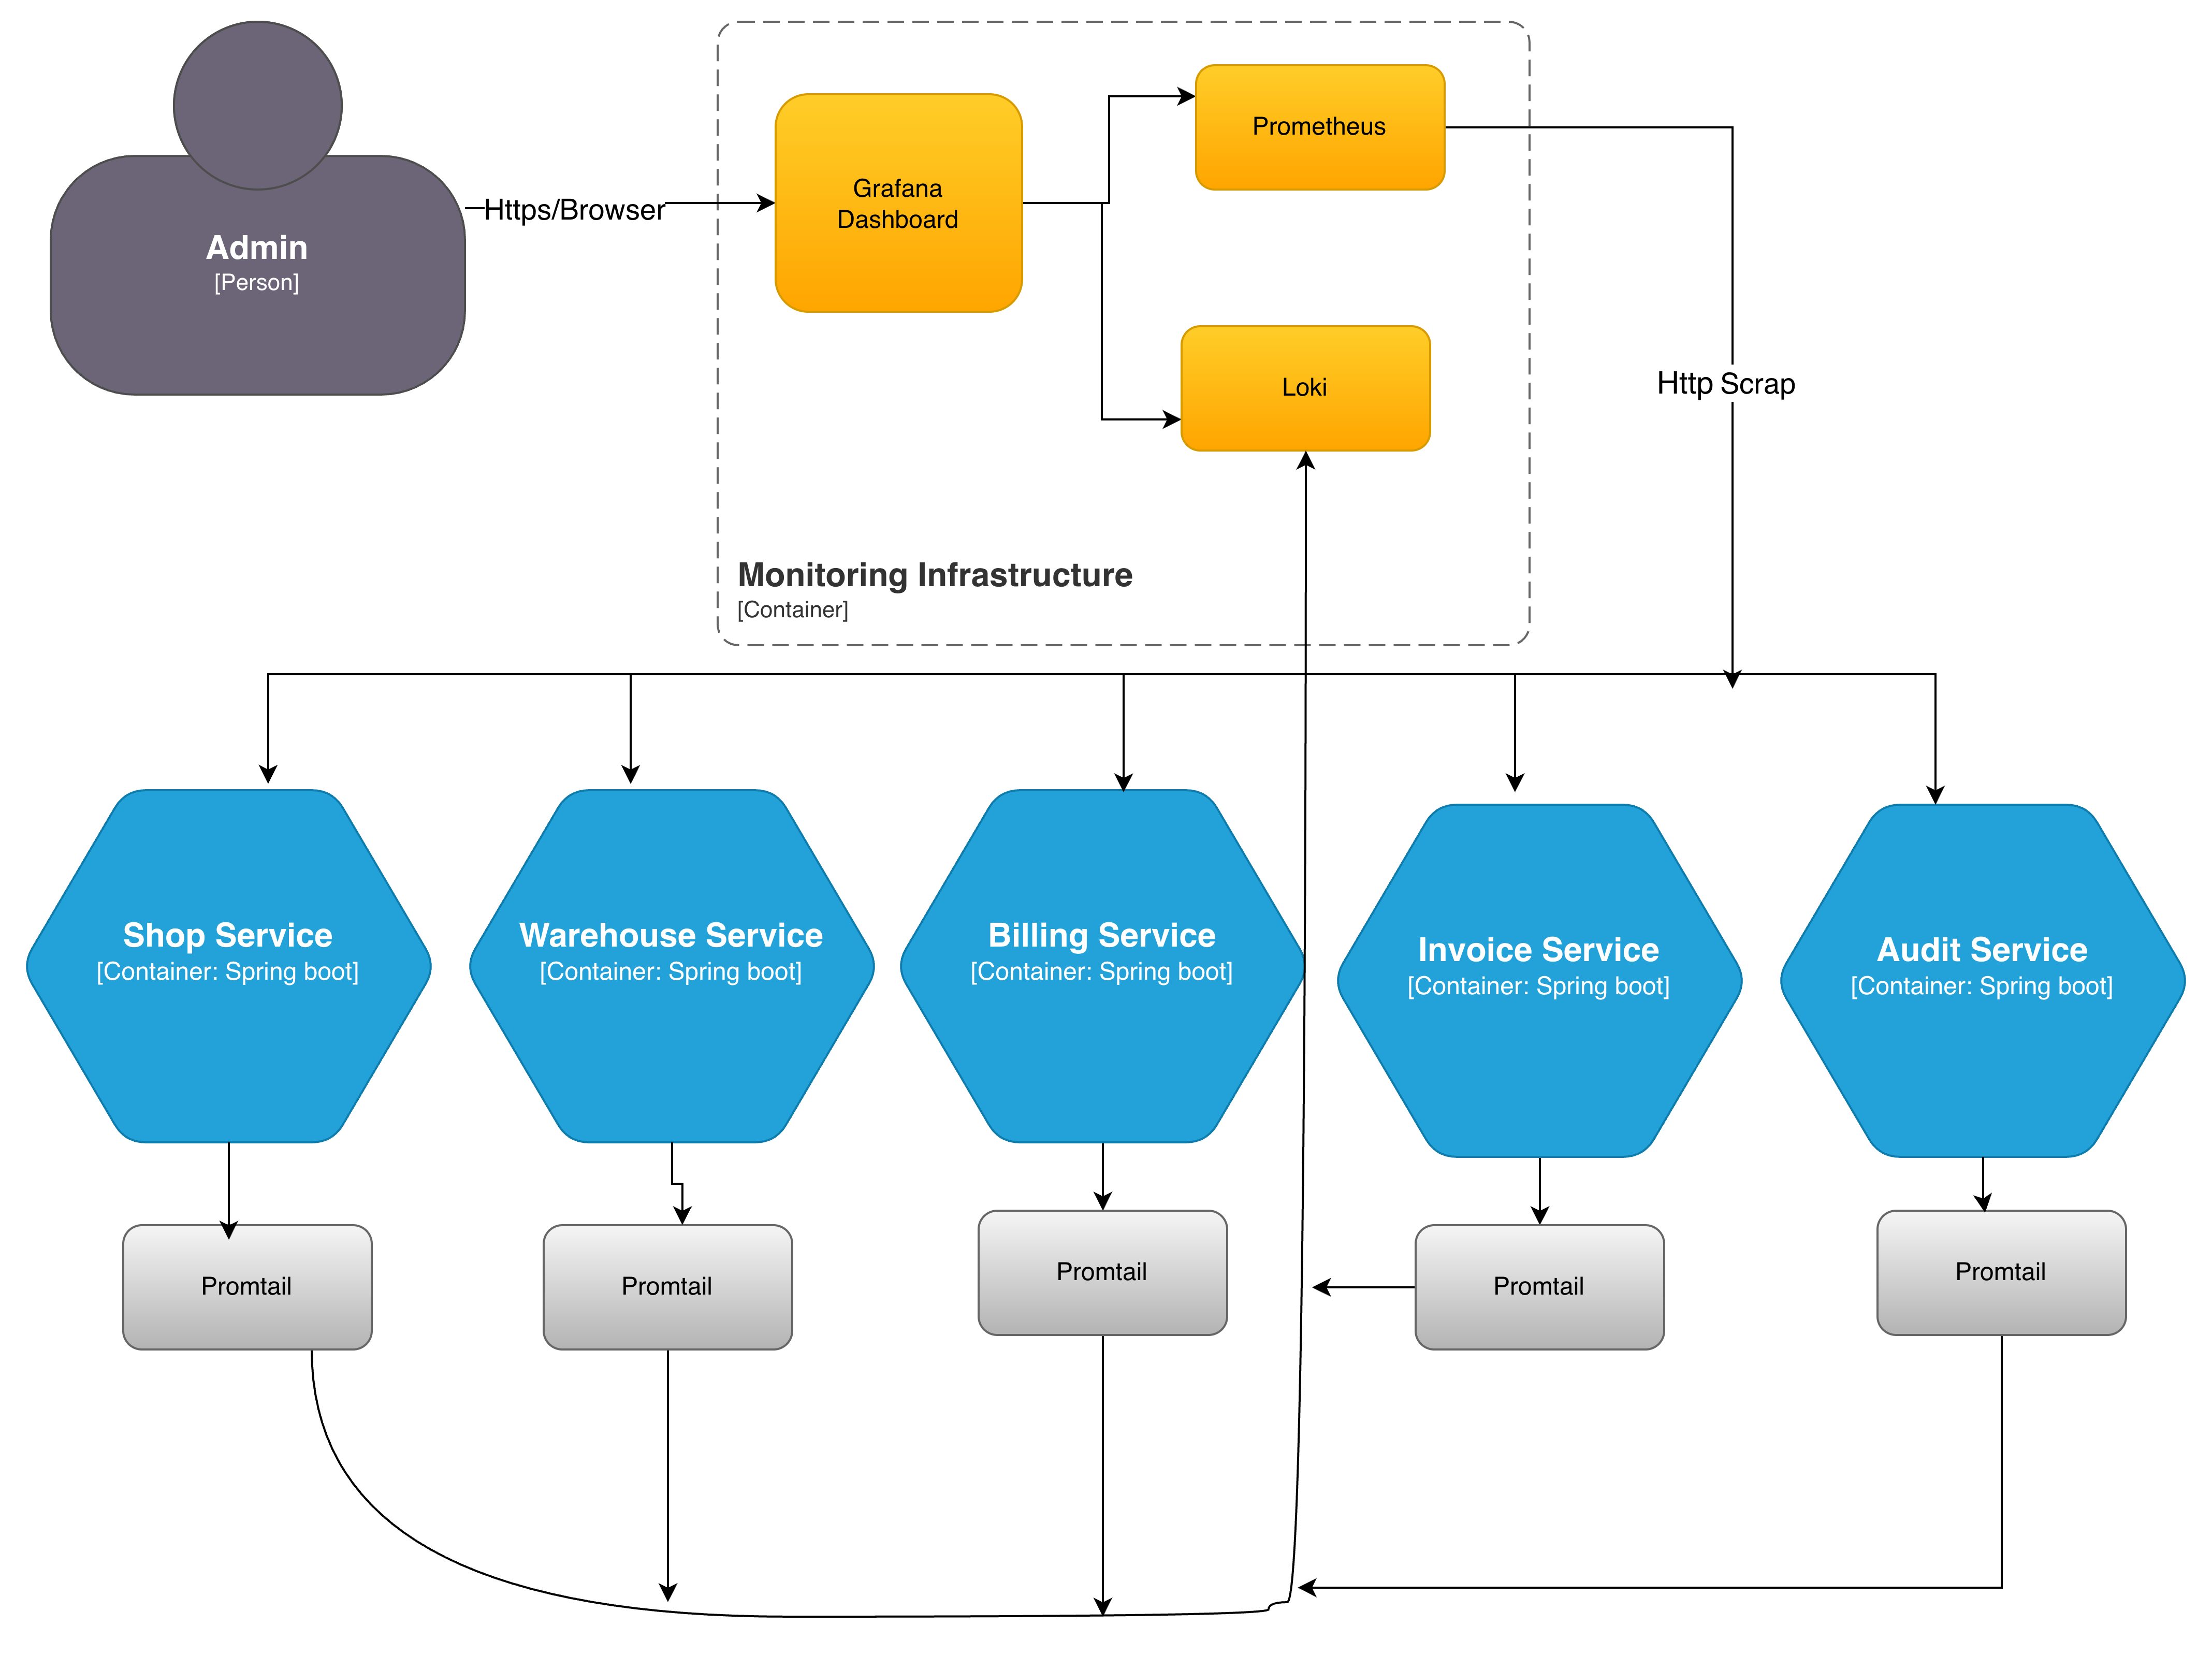
\includegraphics[width=0.78\textwidth,height=0.52\textheight,keepaspectratio]{../images/monitoring.png}
  \caption{Technische Beobachtbarkeit mit Promtail, OpenTelemetry, Loki und Grafana}
  \label{fig:monitoring}
\end{figure}

\section{Aufgabenverteilung}

Abdelwadoud Mabrouk  verantwortete die Entwicklung des Warehouse-, Invoice- und Audit-Services einschließlich Datenhaltung, Kafka-Anbindung und Tests. Im Angular-Frontend übernahm er das initiale Setup des Projekts, die Implementierung des Audit-Dashboards sowie die Administration und Rechteverwaltung (Login, Admin- und User-Bereich). Zudem lagen die Einrichtung der Observability (Monitoring/Logging) sowie das Aufsetzen der initialen Dokumentationsstruktur in seinem Aufgabenbereich.

Mohammed Amine Grioui verantwortete den \textit{Shop-} und \textit{Billing-Service} sowie den Frontend-Checkout. Sein Backend-Bereich umfasste die Bestell- und Zahlungsorchestrierung über REST und Apache Kafka (Event-Verarbeitung, Topic-Design, Idempotenz). Hierbei konzipierte er das Saga-Design des zentral steuernden \textit{Shop-Services}, welcher die einzelnen Prozessschritte koordiniert. Neben Account-Setup, Evaluierung und Dokumentation von Stripe und PayPal entwarf er eine ngrok-Teststrategie zur Webhook-Validierung gegen reale Sandbox-Umgebungen. Im Frontend entwickelte und integrierte er die Checkout-Benutzeroberflächen.

Zentrale Architekturentscheidungen, die Definition der Event-Verträge, das Tracing mittels Correlation-ID, die Bereitstellung via Docker Compose sowie die serviceübergreifende Integration und die Validierung der End-to-End-Abläufe erarbeiteten und prüften beide Projektmitglieder gemeinsam. Auch die technische Dokumentation wurde gemeinsam finalisiert, wobei jeder Entwickler die Dokumentation für seine jeweils verantworteten Services verfasste.

\chapter{Tests}

Im Anschluss an die Implementierung war die Zuverlässigkeit des Gesamtsystems unter realen Fehlerbedingungen zu validieren. Hierfür kombiniert das Testkonzept feingranulare Komponententests mit durchgängigen Ende-zu-Ende-Prüfungen der verteilten Systemarchitektur.

\section{Teststrategie}

Unit-Tests prüfen einzelne Regeln und Use Cases. Integrationstests prüfen die
Zusammenarbeit mit Datenbank oder Kafka. Die .NET-End-to-End-Tests prüfen das Zusammenspiel von Warehouse-, Invoice- und Audit-Service über REST und Kafka. Sie ersetzen keinen vollständigen Browser-basierten Test des gesamten Systems einschließlich Angular, Shop und Billing.

Die Tests orientieren sich am sichtbaren Verhalten. Sie prüfen Zustände,
Idempotenz und Fehlerreaktionen, nicht nur interne Methoden.

\section{Integrationstests des Bestellprozesses}

Um die Fehlertoleranz und das Zusammenspiel der Services unter realistischen Bedingungen zu validieren, setzen wir im \texttt{ShopService} auf Integrationstests mit \texttt{@SpringBootTest} und \texttt{MockMvc}. Externe Abhängigkeiten wie der Warehouse- und der Billing-Service werden dabei mithilfe von \textbf{WireMock} simuliert. Dadurch können wir sowohl erfolgreiche Durchläufe als auch komplexe Fehlerszenarien deterministisch testen.

\subsection{Happy Path}
Im Erfolgsfall durchläuft die Bestellung den gesamten Lebenszyklus:
\begin{enumerate}
    \item Das Warehouse reserviert den Bestand erfolgreich.
    \item Der Billing-Service initiiert den Zahlungsablauf.
    \item Die Bestellung wechselt in den Zustand \texttt{AWAITING\_PAYMENT} und liefert den Status \texttt{201 Created} inklusive Weiterleitungs-URL zurück.
\end{enumerate}
Der Test verifiziert hierbei nicht nur die HTTP-Antwort, sondern stellt auch sicher, dass die Daten korrekt in der Datenbank abgelegt und die externen Schnittstellen exakt einmal aufgerufen wurden.

\subsection{Fehlerszenarien und Resilienzmuster}
Ein zentraler Schwerpunkt der Tests liegt auf der Überprüfung des Systemverhaltens bei Teilausfällen (Saga-Pattern und Retry-Mechanismen):

\begin{itemize}
    \item \textbf{Fehlender Lagerbestand (409 Conflict):} Antwortet das Warehouse mit einem fachlichen Fehler (kein Bestand), bricht der Prozess sofort ab. Es wird kein Aufruf an den Billing-Service getätigt und der Bestellstatus wechselt direkt auf \texttt{OUT\_OF\_STOCK}.

    \item \textbf{Ausfall des Billing-Service \& Saga-Kompensation (503 Service Unavailable):} Fällt der Billing-Service aus, greift die konfigurierte Resilience-Strategie (\texttt{Resilience4j}). Das System führt automatisch gestaffelte Wiederholungsversuche (Exponential Backoff) durch. Schlagen alle Versuche fehl, greift das \textbf{Saga-Pattern zur Kompensation}: Bereits getätigte Reservierungen im Warehouse werden über einen \texttt{DELETE}-Aufruf wieder storniert, der Bestellstatus wechselt auf \texttt{PAYMENT\_FAILED} und der Client erhält ein sauberes HTTP 503-Feedback.


    \item \textbf{Unerreichbarkeit des Warehouse-Service (503 Service Unavailable):} Fällt das Warehouse bereits zu Beginn aus, greift ebenfalls der Retry-Mechanismus. Nach Fehlschlag bricht die Transaktion ab, ohne dass nachgelagerte Billing-Aufrufe oder Stornierungen ausgelöst werden.
\end{itemize}


\section{Automatisierte Ergebnisse}

Der aktuelle .NET-Stand umfasst 40 Unit-Tests und fünf End-to-End-Tests. Alle
45 Tests laufen erfolgreich.

\begin{table}[H]
  \centering
  \caption{Automatisierte Tests des .NET-Anteils
  \label{tab:tests}}
  \begin{tabularx}{0.78\textwidth}{Xr}
    \toprule
    Testbereich & Bestanden \\
    \midrule
    Audit-Service & 10 \\
    Warehouse-Service & 18 \\
    Invoice-Service & 12 \\
    End-to-End & 5 \\
    \midrule
    Gesamt & 45 \\
    \bottomrule
  \end{tabularx}
\end{table}

Die wichtigsten Szenarien sind der Happy Path, fehlender Bestand und parallele
Reservierungen. Weitere Tests senden \texttt{PAYMENT\_SUCCEEDED} doppelt oder
übergeben ein ungültiges Event. Dabei entstehen trotzdem nur eine Reservierung
und eine Rechnung. Der Ablauf nach \texttt{PAYMENT\_FAILED} gehört nicht zu
diesen fünf automatisierten .NET-End-to-End-Tests.

\section{Manuelle Prüfung}

Zusätzlich haben wir geprüft, ob der technische Ablauf auch über die
Benutzeroberfläche nachvollziehbar bleibt. Dazu öffneten wir Produktkatalog,
Checkout, Lager, Rechnungsübersicht, Audit-Timeline, Systemstatus und Grafana im
laufenden Docker-Stack.

\chapter{Ergebnis}

\section{Erreichte Ziele}

Das Projekt setzt eine verteilte E-Commerce-Plattform mit klaren Domänengrenzen um. Fehlgeschlagene Transaktionen werden über das Saga-Pattern deterministisch zurückgerollt, während Idempotenz-Mechanismen vor Doppelverarbeitungen schützen. Das Gesamtsystem startet reproduzierbar via Docker Compose und bietet durch die Kombination aus Audit-Timeline und Log-Aggregation (Loki, Grafana, OpenTelemetry) umfassende fachliche und technische Beobachtbarkeit.

\section{Erweiterbarkeit}

Die Architektur ermöglicht eine einfache Skalierung und Erweiterung:
\begin{itemize}
    \item \textbf{Zahlungsanbieter:} Neue Anbieter lassen sich über die Payment-Fassade ohne Änderungen am Rest des Systems integrieren.
    \item \textbf{Event-Driven Scaling:} Neue Services können bestehende Kafka-Topics autonom konsumieren, ohne Anpassungen an den Publishern zu erfordern.
    \item \textbf{Datenhoheit:} Gemäß \textit{Database-per-Service} bleibt jeder Dienst unabhängig erweiterbar.
\end{itemize}
Die übergreifenden Vorgaben (Datenhoheit, Event-Schemas, Correlation-ID) sind zentral in der \texttt{docs/architecture.md} dokumentiert.

\chapter{Fazit}

Die Konzeption des verteilten E-Commerce-Systems belegt, dass die inhärente Komplexität Microservice-basierter Architekturen primär aus der fehlerresistenten Orchestrierung der Zustandsübergänge zwischen den Domänen resultiert.

Es lässt sich bilanzieren, dass explizite Datenkontrakte, durchgängige Idempotenz sowie reproduzierbare Integrations-Tests das Fundament für die Systemstabilität bilden. Der hybride Kommunikationsansatz – bestehend aus synchronem REST für zustandsrelevante Kaufentscheidungen und ereignisgesteuertem Kafka-Publishing für entkoppelte Nachfolgeschritte – gewährleistet eine saubere funktionale Deaggregation. Eine konsistente \textit{Correlation-ID} sichert hierbei die Traceability über heterogene Service-Grenzen hinweg.

Durch die strikte Datenautonomie der Dienste bleibt die Systemarchitektur auch bei steigender Domänenkomplexität skalierbar und wartbar. Der mittels Docker Compose deterministisch replizierbare Gesamtzustand erfüllt die Anforderungen des Hochschulprojekts vollumfänglich und markiert die Ausgangslage für eine schrittweise Überführung in eine produktive Enterprise-Infrastruktur.

\printbibliography[heading=bibintoc,title={Literaturverzeichnis}]

\end{document}
